\section{TagController Class Reference}
\label{classTagController}\index{TagController@{TagController}}
Inheritance diagram for TagController:\nopagebreak
\begin{figure}[H]
\begin{center}
\leavevmode
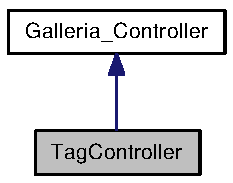
\includegraphics[width=74pt]{classTagController__inherit__graph}
\end{center}
\end{figure}
Collaboration diagram for TagController:\nopagebreak
\begin{figure}[H]
\begin{center}
\leavevmode
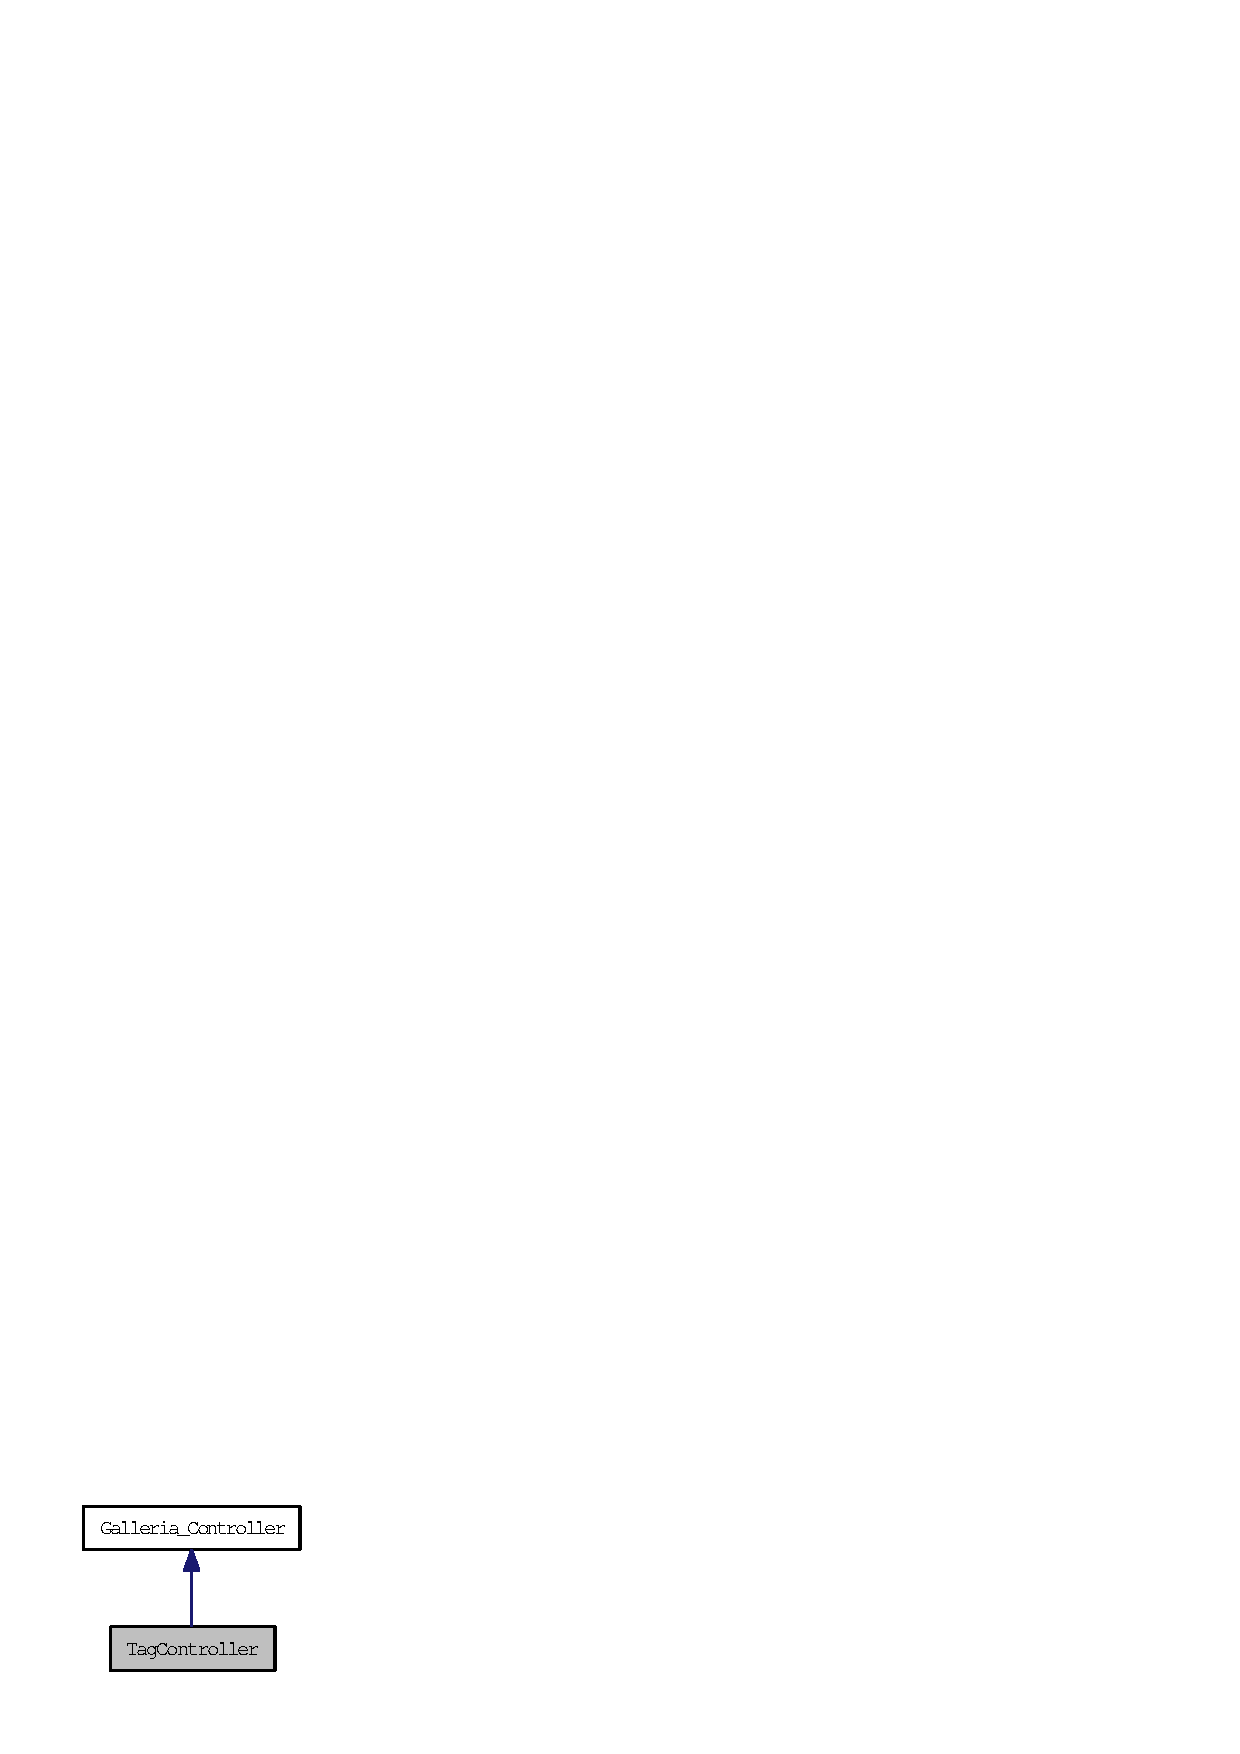
\includegraphics[width=74pt]{classTagController__coll__graph}
\end{center}
\end{figure}
\subsection*{Public Member Functions}
\begin{CompactItemize}
\item 
{\bf indexAction} ()
\end{CompactItemize}


\subsection{Detailed Description}


Definition at line 19 of file tagcontroller.php.

\subsection{Member Function Documentation}
\index{TagController@{TagController}!indexAction@{indexAction}}
\index{indexAction@{indexAction}!TagController@{TagController}}
\subsubsection{\setlength{\rightskip}{0pt plus 5cm}TagController.indexAction ()}\label{classTagController_3fc537f4d4a5b09ee8608a508151d6cc}


Index page.

Index page action. Sets up Tag index page.  public 

Definition at line 28 of file tagcontroller.php.

References Galleria\_\-Controller.\_\-getModel(), and Galleria\_\-Controller.getView().

Here is the call graph for this function:\nopagebreak
\begin{figure}[H]
\begin{center}
\leavevmode
\includegraphics[width=187pt]{classTagController_3fc537f4d4a5b09ee8608a508151d6cc_cgraph}
\end{center}
\end{figure}


The documentation for this class was generated from the following file:\begin{CompactItemize}
\item 
/var/www/galleria/data/site/mvc/controller/{\bf tagcontroller.php}\end{CompactItemize}
